\documentclass[10pt]{beamer}
%\usepackage[utf8]{inputenc}
\usepackage{multirow,rotating}
%\usepackage{color}
%\usepackage{hyperref}
\usepackage{tikz-cd}
\usepackage{array}
\usepackage{siunitx}
\usepackage{mathtools,nccmath}%
\usepackage{
	%etoolbox, 
	xparse} 
\usetheme{CambridgeUS}
\usecolortheme{dolphin}
\usepackage{longtable}
\usepackage{gensymb}
\usepackage{tabularray}
\UseTblrLibrary{booktabs}


% set colors
\definecolor{myNewColorA}{RGB}{158, 27,50}
\definecolor{myNewColorB}{RGB}{158, 27,50}
\definecolor{myNewColorC}{RGB}{158, 27,50} % {130,138,143}
\setbeamercolor*{palette primary}{bg=myNewColorC}
\setbeamercolor*{palette secondary}{bg=myNewColorB, fg = white}
\setbeamercolor*{palette tertiary}{bg=myNewColorA, fg = white}
\setbeamercolor*{titlelike}{fg=myNewColorA}
\setbeamercolor*{title}{bg=myNewColorA, fg = white}
\setbeamercolor*{item}{fg=myNewColorA}
\setbeamercolor*{caption name}{fg=myNewColorA}
\usefonttheme{professionalfonts}
%\usepackage{natbib}
\usepackage{hyperref}
%------------------------------------------------------------
%\titlegraphic{
\includegraphics[height=0.75cm]{iitb1.png}} 

\usepackage[style=verbose,backend=biber]{biblatex}
\addbibresource{\jobname.bib}

\titlegraphic{%
	
\includegraphics[width=3.0cm]{IITB.png}
}

\setbeamerfont{title}{size=\large}
\setbeamerfont{subtitle}{size=\small}
\setbeamerfont{author}{size=\small}
\setbeamerfont{date}{size=\footnotesize}
\setbeamerfont{institute}{size=\footnotesize}
\title[]{Process Simulation using DWSIM \\ A Free and Open Source Chemical Process Simulator}%title
%\subtitle{ }%%subtitle
%\author[Priyam Nayak]{Priyam Nayak - 214026014\inst{1}}%%authors
\author[Priyam Nayak]{Priyam Nayak}
%\institute[IITB]{Indian Institute of Technology Bombay\inst{1}}
\institute[IITB]{Indian Institute of Technology Bombay}
\date[\textcolor{white}{DWSIM Workshop}]
{DWSIM Workshop \\ Mar 19, 2023}

%------------------------------------------------------------
%This block of commands puts the table of contents at the 
%beginning of each section and highlights the current section:
%\AtBeginSection[]
%{
	%  \begin{frame}
		%    \frametitle{Contents}
		%    \tableofcontents[currentsection]
		%  \end{frame}
	%}
\AtBeginSection[]{
	\begin{frame}
		\vfill
		\centering
		\begin{beamercolorbox}[sep=8pt,center,shadow=true,rounded=true]{title}
			\usebeamerfont{title}\insertsectionhead\par%
		\end{beamercolorbox}
		\vfill
	\end{frame}
}
% ------Contents below------
%------------------------------------------------------------

\begin{document}
	
	%The next statement creates the title page.
	\frame{\titlepage}
	\begin{frame}
		\frametitle{Outline}
		\tableofcontents
	\end{frame}
	
	
	% consider removing it if it's too redundant
	\AtBeginSection[]
	{
		\begin{frame}
			\frametitle{Table of Contents}
			\tableofcontents[currentsection]
		\end{frame}
	}

\section{Design, Simulation \& Optimization}
 \begin{frame}{Design, Simulation \& Optimization}
	\begin{figure}
		\centering
		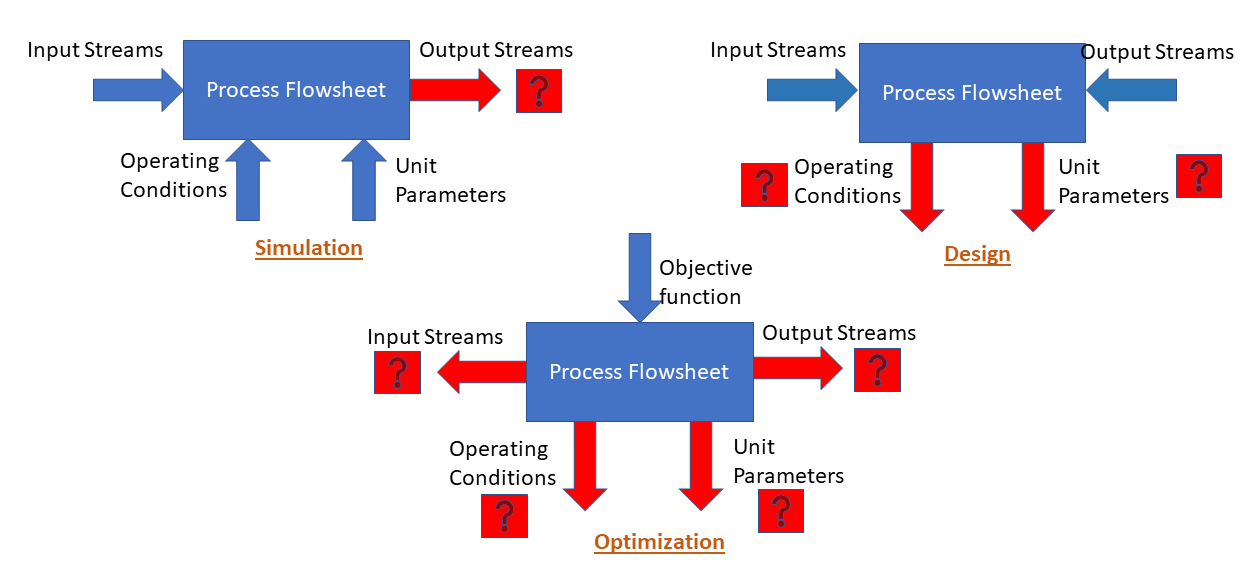
\includegraphics[width=1\linewidth]{des-sim-opt.png}
	\end{figure}
\end{frame}

\section{Simulating a Process Flowsheet}
 \begin{frame}{Simulating a Process Flowsheet}
	\begin{figure}
		\centering
		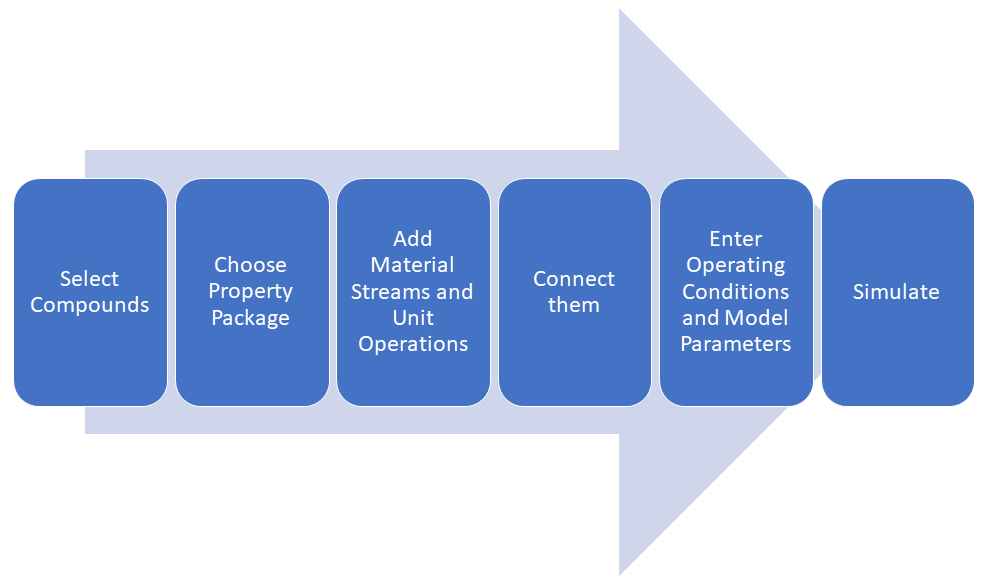
\includegraphics[width=1\linewidth]{flowsheet-seq.png}
	\end{figure}
\end{frame}

\section{Simulating a Material Stream}
\begin{frame}{Simulating a Material Stream}
Important Properties to be specified in a Material Stream
\begin{itemize}
	\item Flash Specification
		\item Flowrate
	\item Composition
\end{itemize}	
\end{frame}

\begin{frame}{Flash Specification}
Flash Properties - Pressure, Temperature, Enthalpy, Entropy, Vapor Fraction
\vspace{3ex}
	\begin{itemize}
		\item Pressure and Temperature (TP)
		\item Pressure and Enthalpy (PH)
		\item Pressure and Entropy (PS)
		\item Pressure and Vapor Fraction (PVF)
		\item Temperature and Vapor Fraction (TVF)
	\end{itemize}	
\end{frame}

\begin{frame}{Flow Rate}
	\begin{itemize}
		\item Mass Flow Rate
		\item Molar Flow Rate
		\item Volumetric Flow Rate
	\end{itemize}	
\end{frame}

\begin{frame}{Composition}
	\begin{itemize}
		\item Mass Fraction
		\item Mole Fraction
		\item Mass Flows of Components
		\item Mole Flows of Components
		\item Molarities
		\item Molalities
	\end{itemize}	
\end{frame}

\section{Simulation of a Flash Separator}
\begin{frame}
\frametitle{Problem 1: Simulation of a Flash Drum or Gas Liquid Separator}
A 100 kmol/hr feed consisting of 10, 20, 30, and 40 mole\% of propane,
n-butane, n-pentane, and n-hexane, respectively, enters a flash chamber
at 15 psia and 50$^\circ$F. The flash drum is operated at 100 psia and 200$^\circ$ F. Applying the Raoult’s law property
package, compute the composition of the exit streams.
\end{frame}


\begin{frame}
	\frametitle{Results: Simulation of a Flash Drum or Gas Liquid Separator}
	\begin{figure}
		\begin{center}
			\includegraphics[width=9cm,height=9cm,keepaspectratio]{flash.png}
		\end{center}
	\end{figure}
\end{frame}

\section{Computation of Bubble Point \& Dew Point}
\begin{frame}
\frametitle{Problem 2: Computation of Bubble Point Temperature}
Compute the bubble point temperature at 18 bar of the following
hydrocarbon mixture using the Soave-Redlich-Kwong property
package. Assume the mixture inlet temperature of 250$^\circ$C, pressure of 5
bar and flow rate of 120 kmol/hr.

\begin{center}
\begin{tabular}{|c|c|}
\hline
Component & Mole Fraction \\ \hline
$C_1$ & 0.05 \\ \hline
$C_2$ & 0.1 \\ \hline
$C_3$ & 0.15 \\ \hline
i-$C_4$ & 0.1 \\ \hline
n-$C_4$ & 0.2 \\ \hline
i-$C_5$ & 0.25 \\ \hline
n-$C_5$ & 0.15 \\ \hline
\end{tabular}
\end{center}

\end{frame}

\begin{frame}
\frametitle{Problem 3: Computation of Dew Point Temperature}
Compute the dew point temperature at 1.5 bar of the following
hydrocarbon mixture using the Soave-Redlich-Kwong property
package. Assume the mixture inlet temperature of 250$^\circ$C, pressure of 5
bar and flow rate of 120 kmol/hr.

\begin{center}
\begin{tabular}{|c|c|}
\hline
Component & Mole Fraction \\ \hline
$C_1$ & 0.05 \\ \hline
$C_2$ & 0.1 \\ \hline
$C_3$ & 0.15 \\ \hline
i-$C_4$ & 0.1 \\ \hline
n-$C_4$ & 0.2 \\ \hline
i-$C_5$ & 0.25 \\ \hline
n-$C_5$ & 0.15 \\ \hline
\end{tabular}
\end{center}

\end{frame}
\section{Generation of VLE Plot}
\begin{frame}
\frametitle{Problem 4: T-xy and P-xy diagrams of a Binary Mixture}

A binary mixture, consisting of 50 mole\% ethanol and 50 mole\% 1-propanol, is fed to a flash drum with a flow rate of 120 kmol/hr at 3.5 bar and 30$^0$C.
\begin{enumerate}
\item Produce T-xy plot at a constant pressure (1.013 bar)
\item Produce P-xy plot at a constant temperature (75$^0$C)
\item Produce xy plot based on the data obtained in Part (2)
\end{enumerate}

Consider the Soave-Redlich-Kwong as a base property method.

\end{frame}

\section{Simulation of Conversion Reactor}
\begin{frame}{Problem Statement}
	100 kg/h of ethyl benzene at 260 \degree C and 1.5 bar is decomposed to form styrene and hydrogen. Products are at 250 \degree C and 1.2 bar. Assume the reaction to be vapour phase and 80\% conversion of ethyl benzene takes place. Using Peng-Robinson model of thermodynamics, simulate the conversion reactor.
	
	\vspace{3ex}
	
	Repeat the above problem with conversion as function of temperature (where T is in K) provided as 
	\begin{equation*}
		f(T) = 0.0425(T+248)
	\end{equation*}
\end{frame}

\begin{frame}{Input Data}
	\begin{itemize}
		\item Components: Ethylbenzene-Styrene-Hydrogen
		\item Thermodynamic Property Package: Peng-Robinson
		\item Feed Mass Flow Rate: 100 kg/hr
		\item Feed Pressure: 1.52 bar
		\item Feed Temperature: 260$^\circ$C
		\item Mole Fraction of Ethylbenzene: 1
		\item Mole Fraction of Styrene: 0
		\item Mole Fraction of Hydrogen: 0
	\end{itemize}
\end{frame}

\begin{frame}{Reaction and Reactor Input}
	\begin{itemize}
		\item Reaction: Ethylbenzene \rightarrow Styrene + Hydrogen
		\item $X_{ethylbenzene}$: 80
		\item Reactor Outlet Temperature: 250$^\circ$C
		\item Reactor Pressure Drop: 0.3 bar
	\end{itemize}
\end{frame}


\section{Simulation of Kinetic Reactor}
\begin{frame}{Problem Statement}
	2000 kg/h of feed consisting of pure acetone at 100 \degree C and 2 bar enters a plug flow reactor (volume of 200 $m^3$ and 10 $m$ length) to decompose into ketene and methane. The reaction rate is 
	\begin{equation*}
		-r_A = kP_{acetone} \frac{kmol}{m^3.hr}
	\end{equation*}
	where $P_{acetone}$ is the partial pressure of the Acetone in $Pa$. The reaction is assumed to follow arrhenius rate law where the pre-exponential factor is equal to 0.916 $hr^{-1}$ and the activation energy is equal to
	45000 $\frac{kJ}{kmol}$. The reactor is operated at 150 \degree C. Assuming the reaction to be in vapor phase and following
	Peng-Robinson property package, simulate a PFR.
\end{frame}

\begin{frame}{Input Data}
	\begin{itemize}
		\item Components: Acetone-Ketene-Methane
		\item Thermodynamic Property Package: Peng-Robinson
		\item Feed Mass Flow Rate: 2000 kg/hr
		\item Feed Pressure: 2 bar
		\item Feed Temperature: 100$^\circ$C
		\item Mole Fraction of Acetone: 1
		\item Mole Fraction of Ketene: 0
		\item Mole Fraction of Methane: 0
	\end{itemize}
\end{frame}

\begin{frame}{Reaction and Reactor Input}
	\begin{itemize}
		\item Reaction: Acetone \rightarrow Ketene + Methane
		\item Pre-exponential factor: 0.916 $hr^{-1}$
		\item Activation Energy: 45000 $\frac{kJ}{kmol}$
		\item Reactor Volume: 200 $m^3$
		\item Reactor Length: 10 m
		\item Reactor Outlet Temperature: 150$^\circ$C
	\end{itemize}
\end{frame}

\section{Simulation of Binary Column Distillation}
\begin{frame}{Problem Statement}
	A 10000 kg/hr feed consisting 40\% (by mole) Benzene and 60\% Toluene enters a distillation column at 1.01325 bar and 80$^\circ$C. The feed is to be separated such that composition of light key in bottoms is 1\% (by mole) and composition of heavy key is 1\% (by mole) in distillate. The
	column is operated at 1.4 times the minimum reflux ratio. The toal condenser pressure is 1.01325 bar and reboiler
	pressure is 1.01325 bar. Using Peng-Robinson property package, simulate the distillation column.
\end{frame}

\begin{frame}{Input Data}
	\begin{itemize}
		\item Components: Benzene-Toluene
		\item Thermodynamic Property Package: Peng-Robinson
		\item Feed Mass Flow Rate: 10000 kg/hr
		\item Feed Pressure: 1.01325 bar
		\item Feed Temperature: 80$^\circ$C
		\item Mole Fraction of Benzene: 0.4
		\item Mole Fraction of Toluene: 0.6
	\end{itemize}
\end{frame}

\begin{frame}{Column Input}
	\begin{itemize}
		\item Mole Fraction of LK(Benzene) in Bottoms: 0.01
		\item Mole Fraction of HK(Toluene) in Distillate: 0.01
		\item Condenser Type: Total
		\item Condenser Pressure: 1.01325 bar
		\item Reboiler Pressure: 1.01325 bar
		\item $\frac{R}{R_{min}}$ = 1.4
	\end{itemize}
\end{frame}


\begin{frame}{Shortcut Column Results}
	\begin{itemize}
		\item Reflux Ratio: 2.19366
		\item Minimum Reflux Ratio: 1.5669
		\item Actual Number of Stages: 19
		\item Feed Stage Location: 9
	\end{itemize}
\end{frame}


\begin{frame}{Distillation Column Input}
	\begin{itemize}
		\item Actual Number of Stages: 19+1
		\item Feed Stage Location: 9
		\item Reflux Ratio: 2.19
		\item Bottoms Flow Rate: 69.5776 kmol/h
	\end{itemize}
\end{frame}

\section{Simulation of Multicomponent Distillation}
\begin{frame}{Problem Statement}
	A 10000 kg/hr feed consisting 50\% (by mole) Benzene, 30\% Toluene and 20\% p-Xylene enters a distillation column at 1.01325 bar and 80$^\circ$C. The feed is to be separated through a sequence of columns such that in the first column, the composition of light key in bottoms is 0.1\% (by mole) and composition of heavy key is 1\% (by mole) in distillate. In the second column, the composition of light key in bottoms is 1\% (by mole) and composition of heavy key is 1\% (by mole) in distillate. The columns are operated at 1.3 times the minimum reflux ratio. For both the columns, the toal condenser pressure is 1.01325 bar and reboiler pressure is 1.01325 bar. Using Peng-Robinson property package, simulate the sequence of distillation column.
\end{frame}

\begin{frame}{Input Data}
	\begin{itemize}
		\item Components: Benzene-Toluene-p-Xylene
		\item Thermodynamic Property Package: Peng-Robinson
		\item Feed Mass Flow Rate: 10000 kg/hr
		\item Feed Pressure: 1.01325 bar
		\item Feed Temperature: 80$^\circ$C
		\item Mole Fraction of Benzene: 0.5
		\item Mole Fraction of Toluene: 0.3
		\item Mole Fraction of P-xylene: 0.2
	\end{itemize}
\end{frame}

\begin{frame}{Column Input}
	\begin{itemize}
		\item Mole Fraction of LK(Benzene) in Bottoms: 0.001
		\item Mole Fraction of HK(Toluene) in Distillate: 0.01
		\item Condenser Type: Total
		\item Condenser Pressure: 1.01325 bar
		\item Reboiler Pressure: 1.01325 bar
		\item $\frac{R}{R_{min}}$ = 1.3
	\end{itemize}
\end{frame}

\begin{frame}{Shortcut Column-I Results}
	\begin{itemize}
		\item Reflux Ratio: 1.31455
		\item Minimum Reflux Ratio: 1.01119
		\item Actual Number of Stages: 26
		\item Feed Stage Location: 16
	\end{itemize}
\end{frame}


\begin{frame}{Distillation Column-I Input}
	\begin{itemize}
		\item Actual Number of Stages: 26+1
		\item Feed Stage Location: 16
		\item Reflux Ratio: 1.31455
		\item Bottoms Flow Rate: 56.3513 kmol/h
	\end{itemize}
\end{frame}


\begin{frame}{Shortcut Column-II Results}
	\begin{itemize}
		\item Reflux Ratio: 1.86416
		\item Minimum Reflux Ratio: 1.43397
		\item Actual Number of Stages: 26
		\item Feed Stage Location: 14
	\end{itemize}
\end{frame}


\begin{frame}{Distillation Column-II Input}
	\begin{itemize}
		\item Actual Number of Stages: 26+1
		\item Feed Stage Location: 14
		\item Reflux Ratio: 1.86
		\item Bottoms Flow Rate: 22.6424 kmol/h
	\end{itemize}
\end{frame}

\section{Simulation of Heat Exchanger}
\begin{frame}
\frametitle{Problem 11: Simulation of Heat Exchanger}
A heat exchanger is to be used to transfer heat to a toluene feed stream from a styrene product stream. The toluene enters the exchanger at a flow rate of 125000 lb/hr at 100$^0$F and 90 psia. The styrene enters at a flow rate of 150000 lb/hr at 300$^0$F and 50 psia. Overall heat transfer coefficient is 55 BTU/[ft$^2$ h R] and the area of the heat exchanger is 3000 ft$^2$. Calculate the fluid outlet temperatures, total heat exchanged, thermal efficiency and LMTD.
\end{frame}

\begin{frame}
\frametitle{Important Links}

FOSSEE DWSIM Webpage: \newline \url{https://dwsim.fossee.in/}

\vspace{3ex}

DWSIM Flowsheeting Project: \url{https://dwsim.fossee.in/flowsheeting-project}

\vspace{3ex}

DWSIM Spoken Tutorials: \url{https://spoken-tutorial.org/tutorial-search/?search_foss=DWSIM&search_language=English}

\vspace{3ex}

DWSIM Developer's Webpage: \url{http://dwsim.inforside.com.br/}

\end{frame}

\begin{frame}
\frametitle{References}
\begin{itemize}
\item Fogler, H. Scott (2005), \textit{Elements of Chemical Reaction Engineering}, 3rd ed., Prentice-Hall of India, New Delhi.
\vspace{2ex}
\item Seider, W.D., J.D. Seider and D.R. Lewin (1998), \textit{Process Design Principles: Synthesis, Analysis, and Evaluation}, 1st ed., John Wiley \& Sons, New York.
\vspace{2ex}
\item Jana, Amiya K. \textit{Process Simulation and Control Using Aspen}, PHI Learning, 2014. 
\end{itemize}

\end{frame}

\begin{frame}
	\begin{center}
		\begin{Huge}
			\textbf{For any queries}
		\end{Huge}
	\end{center}
	\begin{center}
		\begin{Huge}
			contact-dwsim@fossee.in
		\end{Huge}
	\end{center}
\end{frame}


\begin{frame}
\begin{center}
\begin{Huge}
\textbf{Thanks}
\end{Huge}
\end{center}
\begin{center}
\begin{Huge}
for your time and patience
\end{Huge}
\end{center}
\end{frame}

\end{document}